% A Cancellation Method for Hard Special Leaves
% in the Combinatorial Prime Counting Algorithms
% Kim Walisch, October 2026
%
% Build: pdflatex (run three times), or: latexmk -pdf <file>.tex
% Uses only standard packages (amsart, amssymb, mathtools, microtype,
% booktabs, enumitem, xcolor, tikz, hyperref, cleveref) and the
% Computer Modern Type 1 fonts.

\documentclass[11pt,a4paper]{amsart}

\usepackage[a4paper,textwidth=150mm,textheight=246mm,hmarginratio=1:1,headsep=9mm,footskip=12mm]{geometry}
\usepackage{amssymb}
\usepackage{mathtools}
\usepackage[final]{microtype}
\usepackage{booktabs}
\usepackage{array}
\usepackage{enumitem}
\usepackage[section]{placeins}
\usepackage{xcolor}
\usepackage{tikz}
\usetikzlibrary{arrows.meta}

% Take the section sign from the Computer Modern symbol font (OMS), which
% exists as a Type 1 font in every TeX installation; the default TS1 glyph
% requires the cm-super fonts.
\DeclareTextSymbolDefault{\textsection}{OMS}

\definecolor{linkblue}{RGB}{0,62,140}
\definecolor{figblue}{RGB}{38,84,150}
\definecolor{figaccent}{RGB}{176,30,45}

\usepackage[colorlinks=true,linkcolor=linkblue,citecolor=linkblue,urlcolor=linkblue]{hyperref}
\hypersetup{
  pdftitle={A Cancellation Method for Hard Special Leaves in the Combinatorial Prime Counting Algorithms},
  pdfauthor={Kim Walisch},
  pdfsubject={Gourdon's prime counting algorithm: cancellation of prime hard special leaves},
  pdfkeywords={prime counting function, Gourdon's algorithm, hard special leaves,
    partial sieve function, Moebius function, Dirichlet hyperbola method}
}
\usepackage[capitalize,nameinlink]{cleveref}

% This paper contains no lemmas, theorems, proofs or examples.
\numberwithin{equation}{section}

% Notation
\DeclarePairedDelimiter{\floor}{\lfloor}{\rfloor}
\newcommand{\Pminus}{P^{-}}
\newcommand{\Pplus}{P^{+}}
% two-line right-aligned table header
\newcommand{\thead}[2]{\begin{tabular}[b]{@{}r@{}}#1\\#2\end{tabular}}
% run-in heading for the steps of Section 5
\newcommand{\step}[1]{\subsection*{#1}}

\setlist[itemize]{leftmargin=1.6em,itemsep=2pt,topsep=3pt}
\setlist[enumerate]{leftmargin=2.2em,itemsep=2pt,topsep=3pt}

% Slightly less space above the first-page footnotes (date, MSC, keywords).
\addtolength{\skip\footins}{-3pt}
\begin{document}

\title[A cancellation method for hard special leaves]{A Cancellation Method for Hard Special Leaves\\ in the Combinatorial Prime Counting Algorithms}
\author{Kim Walisch}
\dedicatory{with the AI assistants GPT-6 Astra (OpenAI) and Claude Opus 5.5 (Anthropic)}
\date{October 2026}
\subjclass[2020]{Primary 11Y16; Secondary 11A25, 11N05}
\keywords{Prime counting function, Gourdon's algorithm, hard special leaves,
partial sieve function, M\"obius function, Dirichlet hyperbola method}

\begin{abstract}
Chopper Lin has devised a new and substantial
improvement to the computation of the hard special leaves, the formula~$D$ of
Gourdon's prime counting algorithm, and contributed it to the primecount
library in pull request~\#146. To the author's knowledge, the method has not
been published before. Its key idea is to pair, for each sieving prime~$p$, the
partial sieve function $\Phi_p(t)=\phi(t,\pi(p)-1)$ with a M\"obius prefix sum
$M_p(t)$ restricted to integers all of whose prime factors exceed~$p$. For
$p^2\le t<p^3$ their difference is a combination of three values of~$\pi$, and
a weighted Dirichlet hyperbola rearrangement of the top band of leaves in each
eligible row absorbs the leaves above $\sqrt{x/p}$ into boundary terms and gives
every other prime leaf of the band the coefficient $1+\mu(q)=0$, so that its
expensive sieve query cancels exactly. In primecount the method removes $31\%$
of the sieve queries of~$D$ at $x=10^{20}$ and $44\%$ at $x=10^{23}$, and the
pull request implementing it reduces the running time of~$D$ by up to $23.8\%$ in our benchmarks. Because it
relies only on the structure of the special leaves, it should also apply to the
algorithms of Lagarias, Miller and Odlyzko and of Del\'eglise and Rivat whenever
$y>x^{2/5}$. This note derives Lin's method step by step, with all intermediate steps,
explains what each condition is used for, describes how the remaining terms
are evaluated, and sketches a generalization to parameters $z>y$.
\end{abstract}

\maketitle

% ======================================================================
\section{Introduction}\label{sec:intro}

The combinatorial algorithms for the prime counting function $\pi(x)$, from
Meissel and Lehmer~\cite{Lehmer1959} through Lagarias, Miller and
Odlyzko~\cite{LMO1985} and Del\'eglise and Rivat~\cite{DR1996} to
Gourdon~\cite{Gourdon2001}, express $\pi(x)$ through values of the partial sieve
function $\phi(x,a)$, which counts the integers $n\le x$ that are not divisible
by any of the first $a$ primes; see~\cite{OeS2006,Staple2015,Staple2015thesis} for detailed
expositions. The primecount library~\cite{primecount} implements Gourdon's
variant
\begin{equation}\label{eq:gourdon}
  \pi(x)=A-B+C+D+\Phi_0+\Sigma.
\end{equation}
The formulas $A$, $B$ and $C$ reduce to values of~$\pi$, and the ordinary
leaves~$\Phi_0$ to values of $\phi(\cdot,k)$ for a small constant~$k$. The
formula~$D$ of the \emph{hard special leaves} is different: each of its terms
needs a value $\phi(t,b-1)$ that is obtained by counting the unsieved elements
of a segmented sieve~\cite{Walisch2025hard}. At $x=10^{20}$, $D$ accounts for
$52\%$ of the total running time~\cite[\S4]{Lin2026}.

Pull request \#146 to primecount~\cite{PR146}, contributed by Chopper Lin in
October 2026, removes a large part of these sieve counts. For a sieving
prime~$p$, it pairs the partial sieve function $\Phi_p(t)=\phi(t,\pi(p)-1)$ with
the restricted M\"obius prefix sum
\[
  M_p(t)=\sum_{\substack{n\le t\\ \Pminus(n)>p}}\mu(n),
\]
where $\Pminus(n)$ is the least prime factor of~$n$, and it rearranges the top
band of leaves in each eligible row of~$D$ across a hyperbola. The leaves above
$\sqrt{x/p}$ are absorbed into a few boundary terms, and every other prime
leaf~$q$ of the band then has the coefficient $1+\mu(q)=0$, so its sieve count
disappears exactly. What remains are cheap lookups in a table of~$\pi$, a much
shorter list of sieve queries indexed by semiprimes, and two boundary queries
per row. An
accompanying experiment report~\cite{Lin2026} describes how the method was found
and measured.

This note explains the mathematics behind the method. It derives every formula
step by step, with all intermediate steps instead of lemmas and proofs, and
recalls earlier definitions where they are needed. The three key formulas
are~\eqref{eq:E}, a closed formula for $\Phi_p(t)-M_p(t)$ when $p^2\le t<p^3$;
\eqref{eq:final}, the band identity; and~\eqref{eq:primeweight}, the
cancellation of the prime leaves. \Cref{sec:leaves} recalls Gourdon's
formula~$D$ and \cref{sec:functions} introduces the two arithmetic functions;
\cref{sec:cheap,sec:band,sec:cancel} derive the three key formulas.
\Cref{sec:gourdon} shows where the band lies inside~$D$, \cref{sec:remaining}
explains how the remaining terms are evaluated, and \cref{sec:practice} reports
operation counts and running times. \Cref{sec:general} sketches a
generalization to parameters $z>y$, and \cref{sec:prior} relates the method to
earlier work. On a first reading, the optional \cref{sec:deeper}, the
implementation details in \cref{sec:Ep,sec:events,sec:cutoff,sec:arith} and the
historical \cref{sec:prior} can be skipped. All identities in this note have also been checked numerically
with an independent implementation.

% ======================================================================
\section{The hard special leaves}\label{sec:leaves}

\subsection{Notation}
\Cref{tab:notation} lists the general notation used throughout; see
\cite[Ch.~2]{Apostol1976} for the basic properties of the M\"obius function. A
sum over $n\le t$ with real $t\ge0$ runs over the integers $1\le n\le\floor{t}$,
so every summatory function~$F$ in this note satisfies $F(t)=F(\floor{t})$, and
we often use $\floor{\floor{x/p}/m}=\floor{x/(pm)}$. The notation of the method
itself is introduced step by step in the following sections and summarized in
\cref{app:notation}.

\begin{table}[htb]
\caption{General notation.}\label{tab:notation}
\centering
\begin{tabular}{@{}l>{\raggedright\arraybackslash}p{110mm}@{}}
\toprule
Symbol & Meaning\\
\midrule
$p$, $q$, $r$ & primes\\
$p_b$ & the $b$-th prime; by convention $p_0=1$\\
$\pi(t)$ & the number of primes up to~$t$\\
$\floor{t}$ & the greatest integer $\le t$\\
$\mu(n)$ & the M\"obius function: $\mu(1)=1$, $\mu(n)=(-1)^k$ if $n$ is a product
  of $k$ distinct primes, and $\mu(n)=0$ otherwise\\
$\Pminus(n)$ & the least prime factor of~$n$; by convention $\Pminus(1)=+\infty$\\
$\Pplus(n)$ & the greatest prime factor of~$n$; by convention $\Pplus(1)=1$\\
$p$-rough & an integer $n$ with $\Pminus(n)>p$\\
square-free & an integer that is not divisible by the square of any prime\\
semiprime & a product of two primes, which may be equal\\
$\phi(t,a)$ & the partial sieve function: the number of integers $n\le t$ with
  $\Pminus(n)>p_a$\\
\bottomrule
\end{tabular}
\end{table}

\subsection{Gourdon's formula \texorpdfstring{$D$}{D}}\label{sec:gourdonD}
Gourdon's algorithm depends on a small constant~$k$ and on parameters $y$
and~$z$, which we take to be integers with $x^{1/3}<y\le z\le\floor{\sqrt x}$
(Gourdon requires $z<x^{1/2}$; primecount also allows $y=z=\sqrt x$ when $x$ is a
perfect square). The primecount library~\cite{primecount} uses $z=y$ and sets
$y$ to $x^{1/3}$ times a single tuning factor, up to rounding and the bounds
above; by default, this factor is an empirically fitted cubic polynomial in
$\log x$ for $x>10^{11}$. With $x_\star=\max(x^{1/4},x/y^2)$, the hard
special leaves form the sum~\cite[\S2]{Gourdon2001}
\begin{equation}\label{eq:D}
  D=-\sum_{k<b\le\pi(x_\star)}\;\sum_{m}\mu(m)\,
     \phi\Bigl(\Bigl\lfloor\frac{x}{p_b m}\Bigr\rfloor,b-1\Bigr),
\end{equation}
where $m$ runs over the square-free integers with
\begin{equation}\label{eq:leafcond}
  \Pminus(m)>p_b,\qquad \Pplus(m)\le y,\qquad m\le z<p_b m,\qquad m\le x/p_b^3.
\end{equation}
In words: all prime factors of~$m$ are greater than~$p_b$ and at most~$y$,
$m$ lies in a window determined by~$z$, and the last condition, which is
equivalent to $\floor{x/(p_bm)}\ge p_b^2$, makes the leaf \emph{hard}. Together
with $m>p_b$ it gives $p_b^4<x$, hence primecount bounds $b$ by $\pi(x^{1/4})$
instead of $\pi(x_\star)$. The
\emph{easy} leaves with $m>x/p_b^3$ satisfy
$\phi(x/(p_bm),b-1)=\pi(x/(p_bm))-b+2$; they belong to Gourdon's formula~$C$
and are computed with a table of~$\pi$.

\subsection{Rows, leaves and sieve queries}\label{sec:rows}
For a fixed sieving prime $p=p_b$, the inner sum in~\eqref{eq:D} is the
\emph{row} of~$p$, and the integers $m$ satisfying~\eqref{eq:leafcond} are its
\emph{leaves}. The contribution of a leaf to~$D$ is
\begin{equation}\label{eq:leaf}
  -\mu(m)\,\phi\Bigl(\Bigl\lfloor\frac{x}{pm}\Bigr\rfloor,b-1\Bigr).
\end{equation}
Throughout we write
\begin{equation}\label{eq:X}
  X=\floor{x/p},
\end{equation}
so that the leaf needs the value of $\phi(\cdot,b-1)$ at
$t=\floor{x/(pm)}=\floor{X/m}$. We use $X$ because the rearrangement of
\cref{sec:band} is a statement about the hyperbola $mn=X$; $X$ is also the
variable \texttt{xp} of primecount and the $X$ of~\cite{Lin2026}.

The primecount library obtains these values from a segmented sieve of the
interval $[0,\floor{x/z})$, which is $[0,\floor{x/y})$ since primecount uses
$z=y$. For every segment and every~$b$ it counts the unsieved
elements up to each position $\floor{X/m}$ in the segment and then removes the
multiples of~$p_b$~\cite{Walisch2025hard}. We call one such count a
\emph{sieve query}. Counting resumes where the previous count stopped, so
within a segment and a row the positions must be nondecreasing. There are many
sieve queries, about $2.2\cdot10^{10}$ at $x=10^{20}$ (\cref{tab:census}), and
they make~$D$ expensive.

% ======================================================================
\section{Two arithmetic functions}\label{sec:functions}

\subsection{The partial sieve function \texorpdfstring{$\Phi_p$}{Φp}}
Fix $p=p_b$, so that $b=\pi(p)$, and write
\begin{equation}\label{eq:Phi}
  \Phi_p(t)=\phi(t,b-1).
\end{equation}
In a leaf of row~$p$ the argument is $t=\floor{x/(pm)}=\floor{X/m}$, so the
familiar expression~\eqref{eq:leaf} contains exactly
\begin{equation}\label{eq:Phileaf}
  \Phi_p(X/m)=\phi\Bigl(\Bigl\lfloor\frac{x}{pm}\Bigr\rfloor,b-1\Bigr).
\end{equation}
Here $x$ stays fixed while the argument varies with~$m$, and the subscript~$p$
takes over the role of the second argument $b-1$. Since $\phi(t,b-1)$ counts
the integers $n\le t$ that are not divisible by any of the primes
$p_1,\dots,p_{b-1}$, it is a sum of the indicator
\begin{equation}\label{eq:a}
  a_p(n)=\begin{cases}1, & \Pminus(n)\ge p,\\ 0, & \text{otherwise},\end{cases}
  \qquad\text{namely}\qquad
  \Phi_p(t)=\sum_{n\le t}a_p(n).
\end{equation}
Thus $\Phi_p(t)$ counts the integers up to~$t$ that have no prime factor
\emph{smaller} than~$p$; the prime factor~$p$ itself is allowed.

\subsection{The restricted M\"obius prefix sum \texorpdfstring{$M_p$}{Mp}}
The Mertens function
\begin{equation}\label{eq:Mertens}
  M(t)=\sum_{n\le t}\mu(n)
\end{equation}
sums the M\"obius function over \emph{all} positive integers up to~$t$. The new
method uses a restricted version,
\begin{equation}\label{eq:Mp}
  M_p(t)=\sum_{\substack{n\le t\\ \Pminus(n)>p}}\mu(n),
\end{equation}
which omits every integer with a prime factor smaller than \emph{or equal
to}~$p$; the remaining integers, the $p$-rough ones, contribute their signed
M\"obius values. The integer $n=1$ is included, because $\Pminus(1)=+\infty$ and
$\mu(1)=1$. To write $M_p$ in the same way as~$\Phi_p$, we define
\begin{equation}\label{eq:c}
  c_p(n)=\begin{cases}\mu(n), & \Pminus(n)>p,\\ 0, & \text{otherwise},\end{cases}
  \qquad\text{so that}\qquad
  M_p(t)=\sum_{n\le t}c_p(n).
\end{equation}

The two functions differ in two ways: $\Phi_p$ counts every integer whose
prime factors are all $\ge p$ with weight~$1$, while $M_p$ requires all prime
factors to be $>p$ and weights each integer by $\mu(n)\in\{-1,0,1\}$.
\Cref{tab:values} shows both functions for $p=5$.

\begin{table}[htb]
\caption{The integers $n\le30$ with $a_5(n)\ne0$ or $c_5(n)\ne0$. All other
$n\le30$ are divisible by $2$ or~$3$, so that $a_5(n)=c_5(n)=0$. Summing the
rows gives $\Phi_5(30)=10$ and $M_5(30)=-6$.}\label{tab:values}
\centering
\begin{tabular}{@{}lrrrrrrrrrr@{}}
\toprule
$n$ & $1$ & $5$ & $7$ & $11$ & $13$ & $17$ & $19$ & $23$ & $25$ & $29$\\
\midrule
$a_5(n)$ & $1$ & $1$ & $1$ & $1$ & $1$ & $1$ & $1$ & $1$ & $1$ & $1$\\
$c_5(n)$ & $1$ & $0$ & $-1$ & $-1$ & $-1$ & $-1$ & $-1$ & $-1$ & $0$ & $-1$\\
\bottomrule
\end{tabular}
\end{table}

Finally, every leaf~$m$ of row~$p$ is square-free and $p$-rough, so
$\mu(m)=c_p(m)$, and by~\eqref{eq:Phileaf} the contribution~\eqref{eq:leaf}
of the leaf to~$D$ becomes
\begin{equation}\label{eq:leafterm}
  -c_p(m)\,\Phi_p(X/m).
\end{equation}
This is the form in which the leaves will be rearranged.

% ======================================================================
\section{Why the difference \texorpdfstring{$\Phi_p-M_p$}{Φp − Mp} is cheap}\label{sec:cheap}

The first key formula says that for arguments between $p^2$ and~$p^3$ the
difference of the two functions needs only three values of~$\pi$: for
$p^2\le t<p^3$,
\begin{equation}\label{eq:E}
  \boxed{\;\Phi_p(t)-M_p(t)=E_p(t)\coloneqq 2\pi(t)+\pi\bigl(\floor{t/p}\bigr)
  +\pi\bigl(\floor{\sqrt t}\bigr)-4b+2.\;}
\end{equation}
We now see where this comes from.

\subsection{One integer at a time}
By~\eqref{eq:a} and~\eqref{eq:c},
\[
  \Phi_p(t)-M_p(t)=\sum_{n\le t}\bigl(a_p(n)-c_p(n)\bigr),
\]
so we can ask how much each integer $n\le t$ contributes. An integer with a
prime factor smaller than~$p$ has $a_p(n)=c_p(n)=0$ and contributes nothing.
Every other $n\le t$ has all its prime factors $\ge p$, and since $t<p^3$ it
has at most two of them, counted with multiplicity: three such factors would
give $n\ge p^3>t$. This leaves the six types of integers in
\cref{tab:cancel}.

\begin{table}[htb]
\caption{Which integers cancel in $\Phi_p(t)-M_p(t)$? The integers $n\le t$ with
$\Pminus(n)\ge p$, for $p^2\le t<p^3$.}\label{tab:cancel}
\centering
\begin{tabular}{@{}lrrrl@{}}
\toprule
$n$ & $a_p(n)$ & $c_p(n)$ & $a_p(n)-c_p(n)$ & \\
\midrule
$1$ & $1$ & $1$ & $0$ & cancels\\
$p$ & $1$ & $0$ & $1$ & \\
$q$, $q>p$ & $1$ & $-1$ & $2$ & \\
$pq$, $q\ge p$ & $1$ & $0$ & $1$ & \\
$q^2$, $q>p$ & $1$ & $0$ & $1$ & \\
$qr$, $p<q<r$ & $1$ & $1$ & $0$ & cancels\\
\bottomrule
\end{tabular}
\end{table}

The integer~$1$ contributes $1-1=0$. A product $qr$ of two distinct primes
$q,r>p$ has $\mu(qr)=+1$ and therefore also contributes $1-1=0$. Not all
products of two primes cancel, however. A factor equal to~$p$ excludes $pq$
from~$c_p$, because $c_p$ requires all prime factors to be strictly larger
than~$p$, and a square has $\mu(q^2)=0$. The row $pq$ includes $p^2$, while the
row $q^2$ requires $q>p$, so no integer is counted twice.

\subsection{Counting the survivors}
Four types survive, and each of them is counted by a single value of~$\pi$, as
\cref{tab:survivors} shows. The integer $p$ contributes~$1$. The primes
$q\in(p,t]$ number $\pi(t)-\pi(p)=\pi(t)-b$ and contribute~$2$ each. The
products $pq\le t$ with $q\ge p$ correspond to the primes $q\in[p,t/p]$, which
number $\pi(\floor{t/p})-(b-1)$. The squares $q^2\le t$ with $q>p$ correspond to
the primes $q\in(p,\sqrt t]$, which number $\pi(\floor{\sqrt t})-b$.

\begin{table}[htb]
\caption{Contributions of the surviving types to $\Phi_p(t)-M_p(t)$, for
$p^2\le t<p^3$.}\label{tab:survivors}
\centering
\begin{tabular}{@{}ll@{}}
\toprule
Type & Contribution\\
\midrule
$n=p$ & $1$\\
$n=q$, $q>p$ & $2\bigl(\pi(t)-b\bigr)$\\
$n=pq$, $q\ge p$ & $\pi(\floor{t/p})-b+1$\\
$n=q^2$, $q>p$ & $\pi(\floor{\sqrt t})-b$\\
\bottomrule
\end{tabular}
\end{table}

These counts are correct because $t\ge p^2$: then $\floor{t/p}\ge p$ and
$\floor{\sqrt t}\ge p$. For $t<p^2$ the last count would be negative,
and~\eqref{eq:E} indeed fails for every $t<p^2$; it also fails at $t=p^3$,
because the integer $p^3$ has three prime factors. Adding the four
contributions gives
\[
\begin{split}
  \Phi_p(t)-M_p(t)&=1+2\bigl(\pi(t)-b\bigr)+\bigl(\pi(\floor{t/p})-b+1\bigr)
   +\bigl(\pi(\floor{\sqrt t})-b\bigr)\\
  &=2\pi(t)+\pi(\floor{t/p})+\pi(\floor{\sqrt t})-4b+2=E_p(t).
\end{split}
\]

\subsection{Why this is cheap}
The classical way to evaluate a single value $\phi(t,b-1)$ with $p^2\le t<p^3$
classifies the integers by their number of prime
factors~\cite{LMO1985,Lehmer1959}:
\[
  \phi(t,b-1)=\pi(t)-b+2+P_2(t,b-1),\qquad
  P_2(t,b-1)=\sum_{p\le q\le\sqrt t}\bigl(\pi(\floor{t/q})-\pi(q)+1\bigr),
\]
where $P_2(t,b-1)$ counts the products $qr\le t$ of primes $p\le q\le r$; see
also~\cite[\S4]{Walisch2025phi}. This needs one value of~$\pi$ for every
prime~$q$ up to~$\sqrt t$: when the two-prime leaves at $x=10^{18}$ are
expanded in this way, they need $804$ values of~$\pi$ per leaf on average, and
still $52$ in the most favorable range of~$p$~\cite[\S6]{Lin2026}. In the
difference $\Phi_p-M_p$, however, the generic products $qr$ with $p<q<r$, which
make up the bulk of~$P_2$, cancel. Only the degenerate products $pq$ and $q^2$
survive, and each of these two families is counted by a single value of~$\pi$.

\subsection{The reverse substitution}
Algebraically, we could read~\eqref{eq:E} as $\Phi_p=M_p+E_p$. The method uses
it the other way round:
\begin{equation}\label{eq:reverse}
  \boxed{\;M_p(t)=\Phi_p(t)-E_p(t)\qquad(p^2\le t<p^3).\;}
\end{equation}
The reason is that the rearrangement of \cref{sec:band} produces values
of~$M_p$. Formula~\eqref{eq:reverse} turns each of them into a value
of~$\Phi_p$ plus three cheap values of~$\pi$, and these values of~$\Phi_p$
can then be combined with values of~$\Phi_p$ that are already present. The
method thus finds cancellations \emph{across} leaves, instead of trying to
replace each individual sieve query by a potentially expensive computation
of~$M_p$.

% ======================================================================
\section{The key step: rearranging the band}\label{sec:band}

\subsection{The band}
For a row~$p$ let
\begin{equation}\label{eq:band}
  H=\floor{\sqrt X},\qquad U>H \text{ an integer},\qquad L=\floor{X/U}.
\end{equation}
Since $U\ge H+1>\sqrt X$, we have $X/U<\sqrt X$ and hence $L\le H$. We call
the range $L<m\le U$ a \emph{band} and define its \emph{band sum}, modelled
on~\eqref{eq:leafterm}, as
\begin{equation}\label{eq:bandsum}
  D_p(L,U)=-\sum_{L<m\le U}c_p(m)\,\Phi_p(X/m).
\end{equation}
For the bands used in~$D$, \cref{sec:gourdon} shows that this is exactly the
contribution of the band's leaves to~$D$; for now we derive an identity for the
sum itself. Like~$X$, the quantities $H$, $U$ and~$L$ depend on the row~$p$; we suppress
this dependence in the notation. Inside~$D$, $U$ will be the top of the row
(\cref{sec:gourdon}); for now $U$ is any integer larger than~$H$. The last step
of the rearrangement also needs $H\ge p^2$ and $U\le p^3$, which holds for
every band used in~$D$. These bands also satisfy $L\ge p^2$, but that condition is
not needed for the identity itself; it is needed only to identify the band with
hard leaves of~$D$ (\cref{sec:gourdon}). The experiment report~\cite{Lin2026}
writes $A$ for~$L$; we use $L$ to avoid a clash with Gourdon's formula~$A$.

\step{Step 1: Expand the partial sieve count into a sum over integers~\texorpdfstring{$n$}{n}.}
Recall from~\eqref{eq:a} that $\Phi_p(t)=\sum_{n\le t}a_p(n)$. For $t=X/m$
this gives
\[
  \Phi_p(X/m)=\sum_{1\le n\le\floor{X/m}}a_p(n).
\]
Here $n$ is the summation variable: it runs over all integers up
to~$\floor{X/m}$, and $a_p(n)=1$ exactly when $n$ has no prime factor smaller
than~$p$. Substituting this into~\eqref{eq:bandsum} and using
$n\le X/m\iff mn\le X$ gives the double sum
\[
  D_p(L,U)=-\sum_{L<m\le U}c_p(m)\sum_{1\le n\le\floor{X/m}}a_p(n)
  =-\sum_{\substack{L<m\le U,\ n\ge1\\ mn\le X}}c_p(m)\,a_p(n).
\]
The band sum is therefore a weighted sum over the lattice points $(m,n)$ under
the hyperbola $mn=X$, shown in \cref{fig:band}. Summing such a double sum
first along one axis and then along the other is Dirichlet's hyperbola
method~\cite[Ch.~3]{Apostol1976}.

\step{Step 2: Split the \texorpdfstring{$m$}{m}-range at \texorpdfstring{$H=\floor{\sqrt X}$}{H}.}
Because $L\le H<U$, we may write
\[
  D_p(L,U)=-\sum_{L<m\le H}c_p(m)\,\Phi_p(X/m)
  -\sum_{H<m\le U}c_p(m)\,\Phi_p(X/m).
\]
The first sum, the \emph{columns} of \cref{fig:band}, remains unchanged. In
the second sum, $m>H$ means $m\ge H+1>\sqrt X$, so $mn\le X$ forces
$n<\sqrt X$, that is, $n\le H$. This allows us to reverse the order of
summation in the second sum.

\step{Step 3: Exchange the order of summation in the part \texorpdfstring{$m>H$}{m > H}.}
Call the second sum of Step~2
\[
  S=-\sum_{H<m\le U}c_p(m)\,\Phi_p(X/m)
   =-\sum_{H<m\le U}c_p(m)\sum_{n\le X/m}a_p(n).
\]
Thus $S$ is a double sum over the pairs $(m,n)$ with $H<m\le U$ and
$mn\le X$. For each fixed~$n$ these conditions say
$H<m\le\min(U,\floor{X/n})$, and by Step~2 only $n\le H$ occurs. Summing
over~$n$ first gives
\begin{equation}\label{eq:S-exchanged}
  S=-\sum_{1\le n\le H}a_p(n)\sum_{H<m\le\min(U,\floor{X/n})}c_p(m).
\end{equation}
No terms have been approximated or discarded; only the order of summation has
changed.

\step{Step 4: Split at \texorpdfstring{$n=L$}{n = L} and evaluate the inner sums.}
Recall from~\eqref{eq:c} that $M_p(t)=\sum_{m\le t}c_p(m)$. For every upper
bound $V\ge H$, subtracting two prefix sums gives
\[
  \sum_{H<m\le V}c_p(m)=\sum_{m\le V}c_p(m)-\sum_{m\le H}c_p(m)
  =M_p(V)-M_p(H).
\]
In~\eqref{eq:S-exchanged} the upper bound is $V=\min(U,\floor{X/n})$, and
$V\ge H$ because $\floor{X/n}\ge\floor{X/H}\ge H$ for $n\le H$. This upper
bound changes at $n=L=\floor{X/U}$, which gives two cases.

\emph{Case~1: $1\le n\le L$.} Here $n\le L\le X/U$ gives $X/n\ge U$, so the
upper bound is $V=U$ and the inner sum is $M_p(U)-M_p(H)$. It does not depend
on~$n$. Since $\sum_{n\le L}a_p(n)=\Phi_p(L)$, these $n$ contribute
\[
  -\sum_{n\le L}a_p(n)\bigl(M_p(U)-M_p(H)\bigr)
  =-\Phi_p(L)\bigl(M_p(U)-M_p(H)\bigr),
\]
the \emph{rectangle} in \cref{fig:band}.

\emph{Case~2: $L<n\le H$.} Since $n\ge L+1>X/U$, we have $X/n<U$, so the upper
bound is $V=\floor{X/n}$ and the inner sum is $M_p(X/n)-M_p(H)$. It depends
on~$n$, so these $n$ contribute the sum
\[
  -\sum_{L<n\le H}a_p(n)\bigl(M_p(X/n)-M_p(H)\bigr),
\]
the \emph{rows} in \cref{fig:band}. \Cref{tab:ranges} summarizes the two cases.

\begin{table}[htb]
\caption{The two ranges of~$n$ in Step~4.}\label{tab:ranges}
\centering
\begin{tabular}{@{}llll@{}}
\toprule
Range of $n$ & Largest $m$ & Inner sum & In \cref{fig:band}\\
\midrule
$1\le n\le L$ & $U$ & $M_p(U)-M_p(H)$ & rectangle\\
$L<n\le H$ & $\floor{X/n}$ & $M_p(X/n)-M_p(H)$ & rows\\
\bottomrule
\end{tabular}
\end{table}

Adding the two cases yields
\begin{equation}\label{eq:S}
  S=-\Phi_p(L)\bigl(M_p(U)-M_p(H)\bigr)
  -\sum_{L<n\le H}a_p(n)\bigl(M_p(X/n)-M_p(H)\bigr).
\end{equation}

\begin{figure}[t]
\centering
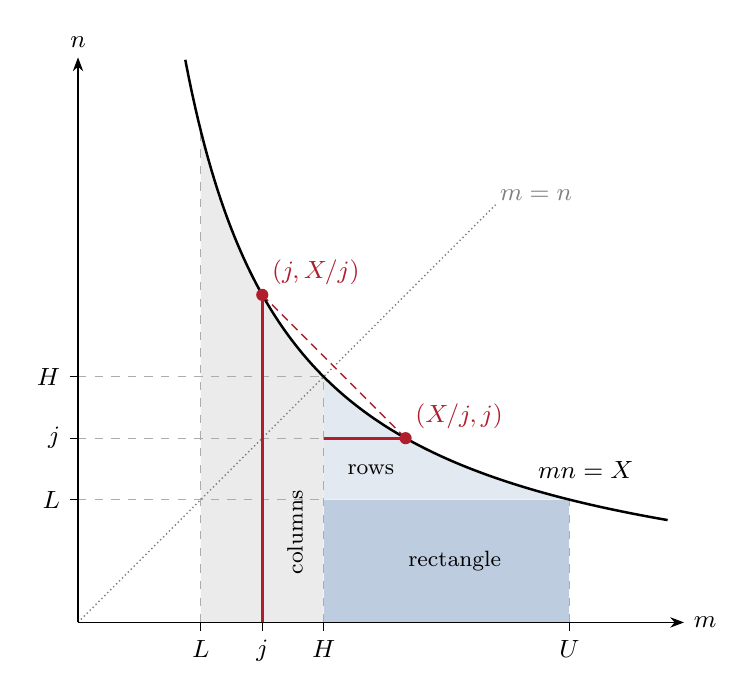
\begin{tikzpicture}[x=0.52cm,y=0.52cm,font=\small,
    guide/.style={gray!65,dashed,line width=0.4pt}]
  \def\vX{36}\def\vL{3}\def\vH{6}\def\vU{12}\def\vk{4.5}\def\vXk{8}
  % regions: kept columns, rectangle and rows
  \fill[gray!16] (\vL,0) -- plot[domain=\vL:\vH,samples=60] (\x,{\vX/\x})
    -- (\vH,0) -- cycle;
  \fill[figblue!30] (\vH,0) rectangle (\vU,\vL);
  \fill[figblue!13] (\vH,\vL) -- plot[domain=\vH:\vU,samples=60] (\x,{\vX/\x})
    -- cycle;
  % guide lines
  \draw[guide] (\vL,0) -- (\vL,{\vX/\vL});
  \draw[guide] (\vH,0) -- (\vH,\vH);
  \draw[guide] (\vU,0) -- (\vU,\vL);
  \draw[guide] (0,\vL) -- (\vH,\vL);
  \draw[guide] (0,\vk) -- (\vH,\vk);
  \draw[guide] (0,\vH) -- (\vH,\vH);
  % diagonal m = n
  \draw[gray,densely dotted,line width=0.5pt] (0,0) -- (10.2,10.2)
    node[above right=-2pt] {$m=n$};
  % axes
  \draw[-{Stealth[length=5pt]}] (0,0) -- (14.8,0) node[right] {$m$};
  \draw[-{Stealth[length=5pt]}] (0,0) -- (0,13.8) node[above] {$n$};
  % hyperbola
  \draw[line width=0.9pt] plot[domain=2.62:14.4,samples=150] (\x,{\vX/\x});
  \node[above right] at (11,{\vX/11}) {$mn=X$};
  % ticks
  \foreach \pos/\lab in {\vL/L,\vk/j,\vH/H,\vU/U}
    \draw (\pos,0) -- (\pos,-0.2) node[below] {$\lab$};
  \foreach \pos/\lab in {\vL/L,\vk/j,\vH/H}
    \draw (0,\pos) -- (-0.2,\pos) node[left] {$\lab$};
  % highlighted column m = j and row n = j
  \draw[figaccent,line width=1.2pt] (\vk,0) -- (\vk,\vXk);
  \draw[figaccent,line width=1.2pt] (\vH,\vk) -- (\vXk,\vk);
  \draw[figaccent,densely dashed,line width=0.5pt] (\vk,\vXk) -- (\vXk,\vk);
  \fill[figaccent] (\vk,\vXk) circle (2.2pt);
  \fill[figaccent] (\vXk,\vk) circle (2.2pt);
  \node[above right,text=figaccent] at (\vk,\vXk) {$(j,X/j)$};
  \node[above right,text=figaccent] at (\vXk,\vk) {$(X/j,j)$};
  % region labels
  \node[rotate=90,font=\footnotesize] at (5.3,2.2) {columns};
  \node[font=\footnotesize] at (9.2,1.5) {rectangle};
  \node[font=\footnotesize] at (7.15,3.72) {rows};
\end{tikzpicture}
\caption{The rearrangement of \cref{sec:band}, drawn schematically for $X=36$ and $U=12$, so
that $H=6$ and $L=3$. The band sum runs over the lattice points $(m,n)$ under
the hyperbola $mn=X$ with $L<m\le U$ (Step~1). The columns $L<m\le H$ are
kept, and the part $m>H$ is summed by rows (Steps~2--4), which yields the
rectangle $n\le L$ and the rows $L<n\le H$. The highlighted column $m=j$ and
row $n=j$ end at the mirror images $(j,X/j)$ and $(X/j,j)$; both need a prefix
value at $X/j$, so in a band that satisfies the conditions of Step~6 they merge
into the weight $a_p(j)+c_p(j)$, which vanishes for prime~$j$.}
\label{fig:band}
\end{figure}

\step{Step 5: Collect the boundary terms.}
Recall from Step~2 that
\[
  D_p(L,U)=-\sum_{L<m\le H}c_p(m)\,\Phi_p(X/m)+S.
\]
Substituting the expression for~$S$ from~\eqref{eq:S} gives
\[
\begin{split}
  D_p(L,U)={}&-\sum_{L<m\le H}c_p(m)\,\Phi_p(X/m)
   -\Phi_p(L)\bigl(M_p(U)-M_p(H)\bigr)\\
  &-\sum_{L<n\le H}a_p(n)\bigl(M_p(X/n)-M_p(H)\bigr).
\end{split}
\]
We expand the brackets and take $M_p(H)$ out of the last sum, since it does not
depend on~$n$:
\[
\begin{split}
  D_p(L,U)={}&-\sum_{L<m\le H}c_p(m)\,\Phi_p(X/m)
   -\Phi_p(L)\,M_p(U)+\Phi_p(L)\,M_p(H)\\
  &-\sum_{L<n\le H}a_p(n)\,M_p(X/n)+M_p(H)\sum_{L<n\le H}a_p(n).
\end{split}
\]
The two positive terms containing $M_p(H)$ combine. By~\eqref{eq:a},
\[
  M_p(H)\Bigl(\Phi_p(L)+\sum_{L<n\le H}a_p(n)\Bigr)=M_p(H)\,\Phi_p(H),
\]
since $\Phi_p(L)$ counts the part up to~$L$ and the sum counts the part from
$L+1$ to~$H$. Finally, we rename $m$ as~$n$ in the first sum and combine the
two sums over $L<n\le H$:
\begin{equation}\label{eq:step5}
\begin{split}
  D_p(L,U)={}&M_p(H)\,\Phi_p(H)-M_p(U)\,\Phi_p(L)\\
  &-\sum_{L<n\le H}\bigl(c_p(n)\,\Phi_p(X/n)+a_p(n)\,M_p(X/n)\bigr).
\end{split}
\end{equation}
Steps~1--5 used nothing about $a_p$ and~$c_p$ except that $\Phi_p$ and $M_p$
are their prefix sums: they are pure bookkeeping, valid for any two arithmetic
functions.

\step{Step 6: Substitute the reverse identity.}
Now the arithmetic of \cref{sec:cheap} enters. Recall from~\eqref{eq:reverse}
that $M_p(t)=\Phi_p(t)-E_p(t)$ for $p^2\le t<p^3$. First we check that this
applies to $t=\floor{X/n}$ for every $L<n\le H$. Since $n\le H$, we have
$t\ge\floor{X/H}\ge H\ge p^2$; since $n>L$, Case~2 of Step~4 showed $t<U\le
p^3$. Hence
\[
  M_p(X/n)=\Phi_p(X/n)-E_p(X/n)\qquad(L<n\le H).
\]
Substituting this into~\eqref{eq:step5}, the boundary terms remain unchanged:
\[
\begin{split}
  D_p(L,U)={}&M_p(H)\,\Phi_p(H)-M_p(U)\,\Phi_p(L)\\
  &-\sum_{L<n\le H}\Bigl(c_p(n)\,\Phi_p(X/n)
   +a_p(n)\bigl(\Phi_p(X/n)-E_p(X/n)\bigr)\Bigr).
\end{split}
\]
Distributing $a_p(n)$ over the parentheses gives
\[
\begin{split}
  D_p(L,U)={}&M_p(H)\,\Phi_p(H)-M_p(U)\,\Phi_p(L)\\
  &-\sum_{L<n\le H}\bigl(c_p(n)\,\Phi_p(X/n)+a_p(n)\,\Phi_p(X/n)
   -a_p(n)\,E_p(X/n)\bigr).
\end{split}
\]
We factor out the shared $\Phi_p(X/n)$ and distribute the outer minus sign.
This gives the final formula for the band:
\begin{equation}\label{eq:final}
  \boxed{\begin{aligned}
  D_p(L,U)={}&M_p(H)\,\Phi_p(H)-M_p(U)\,\Phi_p(L)\\
  &+\sum_{L<n\le H}a_p(n)\,E_p(X/n)
   -\sum_{L<n\le H}\bigl(a_p(n)+c_p(n)\bigr)\,\Phi_p(X/n).
  \end{aligned}}
\end{equation}

% ======================================================================
\section{Why the prime leaves disappear}\label{sec:cancel}

\Cref{sec:cheap} used the difference $a_p(n)-c_p(n)$, in which the products of
two distinct primes greater than~$p$ cancel. In the final
formula~\eqref{eq:final}, the expensive sieve query $\Phi_p(X/n)$ has the
coefficient $a_p(n)+c_p(n)$ instead, and this time the primes cancel. For a
prime $q$ in the band, $L<q\le H$, we have $q>p$ (as $L\ge p^2$ for every band
used in~$D$), and~\eqref{eq:a} and~\eqref{eq:c} give
\begin{equation}\label{eq:primeweight}
  a_p(q)=1,\qquad c_p(q)=\mu(q)=-1,\qquad
  \boxed{\;a_p(q)+c_p(q)=0.\;}
\end{equation}
Consequently the expensive term disappears and only the cheap term remains:
\[
  -\underbrace{\bigl(a_p(q)+c_p(q)\bigr)}_{0}\,\Phi_p(X/q)+a_p(q)\,E_p(X/q)
  =E_p(X/q).
\]

\subsection{The mirror picture}
\Cref{fig:band} shows what happens. The column $m=q$ of the original band
contributes $-c_p(q)\,\Phi_p(X/q)=+\Phi_p(X/q)$. The row $n=q$ created by the
rearrangement contributes, apart from its share of the boundary term
$M_p(H)\,\Phi_p(H)$, the amount $-a_p(q)\,M_p(X/q)=-\Phi_p(X/q)+E_p(X/q)$. The
column ends at the point $(q,X/q)$ and the row at its mirror image $(X/q,q)$;
both need the partial sieve function at the same argument~$X/q$, so the two
sieve queries cancel.

\subsection{The remaining sieve queries}
For the other integers in the band we need \cref{tab:weights}. Since
$p^2\le L<n\le H<p^3$, every $n\in(L,H]$ with $a_p(n)=1$ is either a prime
$q>p^2$ or a product $qr$ of two primes $p\le q\le r$ other than $p^2$ itself.

\begin{table}[htb]
\caption{Coefficients in~\eqref{eq:final} for $L<n\le H$, when $L\ge p^2$ and
$U\le p^3$.}\label{tab:weights}
\centering
\begin{tabular}{@{}lrrrcc@{}}
\toprule
$n$ & $a_p(n)$ & $c_p(n)$ & $a_p(n)+c_p(n)$ & sieve query & $E_p$ term\\
\midrule
$q$ prime & $1$ & $-1$ & $0$ & no & yes\\
$qr$, $p<q<r$ & $1$ & $1$ & $2$ & yes & yes\\
$q^2$, $q>p$ & $1$ & $0$ & $1$ & yes & yes\\
$pq$, $q>p$ & $1$ & $0$ & $1$ & yes & yes\\
$\Pminus(n)<p$ & $0$ & $0$ & $0$ & no & no\\
\bottomrule
\end{tabular}
\end{table}

In other words,~\eqref{eq:final} can be written as
\begin{equation}\label{eq:events}
\begin{split}
  D_p(L,U)={}&M_p(H)\,\Phi_p(H)-M_p(U)\,\Phi_p(L)\\
  &+\sum_{\substack{L<n\le H\\ \Pminus(n)\ge p}}E_p(X/n)
   -\sum_{\substack{L<qr\le H\\ p\le q\le r}}w(q,r)\,\Phi_p\Bigl(\frac{X}{qr}\Bigr),
\end{split}
\end{equation}
where $q$ and $r$ run over primes, $w(q,r)=1$ if $q=p$ or $q=r$, and
$w(q,r)=2$ if $p<q<r$. Apart from the two boundary queries, all sieve
queries that remain in the band are indexed by semiprimes; we call them \emph{semiprime events}. Compared with the original
band sum, the leaves in $(H,U]$ disappear completely, since they are absorbed
into the rectangle and the rows; the prime leaves in $(L,H]$ cancel; the
square-free leaves $qr\in(L,H]$ with $p<q<r$ survive with weight~$2$; and new
sieve queries with weight~$1$ appear at the integers $q^2$ and $pq$ in
$(L,H]$, which are not leaves.

\subsection{A deeper reason (optional)}\label{sec:deeper}
This subsection can be skipped on a first reading. The Dirichlet convolution of
two arithmetic functions is $(f*g)(n)=\sum_{d\mid n}f(d)\,g(n/d)$, and the
Dirichlet series of $f*g$ is the product of the Dirichlet series of $f$
and~$g$~\cite[Ch.~2 and~11]{Apostol1976}. As formal Euler products,
\[
  \sum_{n\ge1}\frac{a_p(n)}{n^s}=\prod_{q\ge p}\bigl(1-q^{-s}\bigr)^{-1},\qquad
  \sum_{n\ge1}\frac{c_p(n)}{n^s}=\prod_{q>p}\bigl(1-q^{-s}\bigr),
\]
so the Dirichlet convolution $a_p*c_p$ is the indicator function of the powers
$1,p,p^2,\dots$. Summing it over $n\le X$ shows that the untruncated analogue
of the band sum collapses:
\[
  \sum_{m\le X}c_p(m)\,\Phi_p(X/m)=\sum_{mn\le X}c_p(m)\,a_p(n)
  =\floor{\log_p X}+1.
\] For a prime $q>p$ this gives
$(a_p*c_p)(q)=a_p(q)+c_p(q)=0$, which is exactly~\eqref{eq:primeweight}. For
$n=qr$ with $p<q<r$ the convolution vanishes as well, but the merged weight is
$a_p(qr)+c_p(qr)=2$, because the cross terms $a_p(q)c_p(r)+a_p(r)c_p(q)=-2$ are
not merged by the rearrangement. This is why only the prime leaves cancel
completely.

% ======================================================================
\section{Where the band sits inside \texorpdfstring{$D$}{D}}\label{sec:gourdon}

\subsection{Which integers in a band are leaves}
Not every band of a row consists of leaves of~$D$. In a band $L<m\le U$ of a
row $p=p_b$ with $k<b\le\pi(x_\star)$, every square-free $p$-rough integer~$m$ is a leaf, provided that
$L\ge p^2$, $U\le y$ and $z<p(L+1)$. Indeed,
$m\le U\le y$ gives $\Pplus(m)\le y$ and $m\le z$; $pm\ge p(L+1)>z$; and
$L\ge p^2$ is equivalent to $U\le\floor{x/p^3}$, which is the hard-leaf
condition $m\le x/p^3$. The band sum $D_p(L,U)$ is then exactly the
contribution of these leaves to~$D$. We restrict bands to $U\le y$,
which guarantees that every square-free $p$-rough integer in the band meets the
condition $\Pplus(m)\le y$; \cref{sec:general} modifies the weight so that this
restriction can be relaxed.

\subsection{The top of the row and the two regions}\label{sec:regions}
By~\eqref{eq:leafcond}, the leaves of row~$p$ satisfy
$z/p<m\le\min(z,\floor{x/p^3})$, and we call $\min(z,\floor{x/p^3})$ the
\emph{top} of the row. When $z=y$, the best choice is to let the band end at the
top, so that the remaining leaves form the single interval $m\le L$. The
implementation~\cite{PR146} does exactly this and distinguishes two
cases:
\begin{itemize}
\item In the \emph{natural region}, $U=\floor{x/p^3}\le y$, together with
$p^2\le U$, $H<U$ and $U<p^3$. Then $L=p^2$ exactly, and
\[
  \Phi_p(L)=\Phi_p(p^2)=\pi(p^2)-b+3,
\]
since the integers counted are~$1$, the primes in $[p,p^2]$, and~$p^2$. The
remaining leaves $m\le p^2$ are all prime, because a composite $p$-rough
integer exceeds~$p^2$: they are the primes in $(\max(p,z/p),p^2]$, and they are
evaluated directly. Here $U$ is the boundary between hard and easy leaves, so this region does
not need $z=y$.
\item In the \emph{$y$-region}, $z=y$ and $\floor{x/p^3}>y$, together with
$H<y$ and $y<p^3$. Then $U=y$ and $L=\floor{X/y}$, and the remaining leaves
$m\le L$ are processed by the ordinary algorithm.
\end{itemize}
\Cref{tab:regions} compares the two regions.

\begin{table}[htb]
\caption{The two regions of band rows.}\label{tab:regions}
\centering
\begin{tabular}{@{}lll@{}}
\toprule
 & natural region & $y$-region\\
\midrule
upper end $U$ & $\floor{x/p^3}\le y$, $U<p^3$ & $y<\floor{x/p^3}$, with $z=y$\\
lower end $L$ & $p^2$ & $\floor{X/y}$\\
precomputed boundary value & $\Phi_p(L)=\pi(p^2)-b+3$ & $M_p(y)$\\
boundary sieve queries & at $H$ and~$U$ & at $L$ and~$H$\\
remaining leaves & the primes in $(\max(p,z/p),p^2]$ & $m\le L$, as before\\
\bottomrule
\end{tabular}
\end{table}

We call the rows of both regions \emph{band rows}. For every band row,
\begin{equation}\label{eq:window}
  p^2\le L\le H<U<p^3,\qquad U\le y,\qquad z<p(L+1),
\end{equation}
so everything in \cref{sec:band,sec:cancel} applies. To see this, note that in
both regions $H<U\le y$ by definition and $L\le H$ by \cref{sec:band}. In the
$y$-region, $\floor{x/p^3}>y$ gives $L\ge p^2$, the condition $U=y<p^3$ is part
of the definition, and $pL\ge p^3>y=z$ gives $z<p(L+1)$. In the natural region
$L=p^2$, and $U<p^3$ is part of the definition. It also gives $z<p^3$, since
$z\ge p^3$ would give $x\ge z^2\ge p^6$ by $z\le\floor{\sqrt x}$, and hence
$U=\floor{x/p^3}\ge p^3$; thus $z<p^3<p(L+1)$. The condition $U<p^3$ must be
checked explicitly: for $p=23$, $x=23^6+1$ and $y=z=23^3=\floor{\sqrt x}$, the
row would otherwise lie in the natural region with $U=p^3$, where~\eqref{eq:E}
does not apply at $t=U$, so that the boundary value $M_p(U)$ of
\cref{sec:remaining} would come out wrong. With $z\le\floor{\sqrt x}-1$, the
bound of primecount before version~9.0, the condition would follow from
$z(y+1)\le z(z+1)<x$. For $z=y$, it also keeps the boundary query at~$U$ below
$\floor{x/y}$, the end of the sieve interval, because $U\le y\le\floor{x/y}$
and $U=\floor{x/y}$ would require $U=y=p^3$. \Cref{tab:hyp} explains what each
condition is used for.

\begin{table}[htb]
\caption{What the conditions on a band are used for.}\label{tab:hyp}
\centering
\begin{tabular}{@{}ll@{}}
\toprule
Condition & Used for\\
\midrule
$H<U$ & splitting at~$H$ in Step~2\\
$H\ge p^2$ and $U\le p^3$ & the reverse substitution in Step~6\\
$L\ge p^2$ & band leaves are hard leaves; only the types of \cref{tab:weights}\\
$U\le y$ and $z<p(L+1)$ & the remaining leaf conditions~\eqref{eq:leafcond}\\
$U<p^3$ & the boundary value $M_p(U)$ (\cref{sec:remaining})\\
\bottomrule
\end{tabular}
\end{table}

\subsection{When do band rows exist?}
Ignoring rounding, the conditions above describe two ranges of sieving primes:
\begin{align*}
  \text{$y$-region:}&\quad \max\bigl(x/y^2,\,y^{1/3}\bigr)<p\le(x/y)^{1/3},\\
  \text{natural region:}&\quad (x/y)^{1/3}\le p<x^{1/5}.
\end{align*}
Indeed, in the $y$-region $H<y$ means $\sqrt{x/p}<y$, that is, $p>x/y^2$;
$L\ge p^2$ means $p\le(x/y)^{1/3}$; and $y<p^3$ means $p>y^{1/3}$. In the natural
region, $U=x/p^3\le y$ means $p\ge(x/y)^{1/3}$, and $H<U$ means $p<x^{1/5}$.
For $y^2<x$, each range is a nonempty interval if and only if $y>x^{2/5}$ (for
$y^2=x$ the $y$-region is empty); an
actual band row also needs a prime in the interval that meets the exact, rounded
conditions. In practice $y>x^{2/5}$ holds by a wide margin: \cref{tab:defaults}
lists primecount's default parameters. With these defaults, band rows first
appeared near $x=4\cdot10^{11}$ in a numerical search and were present at all
larger inputs tested, up to the largest supported input $x=10^{31}$; for
smaller~$x$ the default $y/x^{1/3}$ is below $x^{1/15}$, that
is, $y<x^{2/5}$, and the bands are empty. At $x=10^{20}$ the $969$ band rows lie among the roughly
$1{,}800$ rows with $p\le\sqrt y$, which hold $94\%$ of the sieve queries
of~$D$~\cite[\S6]{Lin2026}. For very large~$x$, the asymptotically optimal
choice $y\asymp x^{1/3}(\log x)^3\log\log x$~\cite[\S2]{Gourdon2001} grows more
slowly than $x^{2/5}$; the band rows then disappear, so the method does not
change the asymptotic complexity of the algorithm.

\begin{table}[htb]
\caption{Default parameters of primecount ($z=y$) and the number of band rows in
the natural region and in the $y$-region.}\label{tab:defaults}
\centering
\begin{tabular}{@{}lrrrr@{}}
\toprule
$x$ & $y/x^{1/3}$ & $y/x^{2/5}$ & natural rows & $y$-region rows\\
\midrule
$10^{12}$ & $7.650$ & $1.212$ & $3$ & $12$\\
$10^{16}$ & $20.871$ & $1.790$ & $37$ & $119$\\
$10^{20}$ & $52.899$ & $2.455$ & $289$ & $680$\\
$10^{24}$ & $140.716$ & $3.535$ & $1{,}992$ & $3{,}659$\\
$10^{28}$ & $321.303$ & $4.368$ & $12{,}196$ & $19{,}165$\\
$10^{31}$ & $539.872$ & $4.630$ & $45{,}118$ & $67{,}681$\\
\bottomrule
\end{tabular}
\end{table}

The $y$-region requires $z=y$ in the current implementation: for $z>y$, a row
can contain further leaves in $(y,\min(z,\floor{x/p^3})]$, namely square-free
$p$-rough integers all of whose prime factors are at most~$y$, and a band ending
at~$y$ then no longer reaches the top of the row. This restriction matters: in
the prototype of~\cite[\S8]{Lin2026}, the natural region alone removed only
$4$--$8\%$ of the sieve queries of~$D$, compared with $23$--$40\%$ for both
regions. Gourdon suggests $z=dy$ with $d>1$~\cite[\S2]{Gourdon2001}; with such a
choice only the natural region would apply, but primecount always uses $z=y$,
which was the fastest setting in the author's benchmarks.
\Cref{sec:general} shows how the $y$-region extends to $z>y$.

% ======================================================================
\section{What still has to be computed}\label{sec:remaining}

For a band row, the computation of~\eqref{eq:events} proceeds as follows; rows
outside the two regions are processed as before.
\begin{enumerate}
\item Compute $X=\floor{x/p}$, $H=\floor{\sqrt X}$, the end~$U$ of the band and
$L=\floor{X/U}$ (\cref{tab:regions}).
\item Add the boundary terms $M_p(H)\,\Phi_p(H)-M_p(U)\,\Phi_p(L)$, which need two
sieve queries (\cref{sec:boundary}).
\item For every prime $q\in(L,H]$, add $E_p(X/q)$; this needs no sieve query
(\cref{sec:Ep}).
\item For every semiprime event $n=qr\in(L,H]$ with primes $p\le q\le r$, add
$E_p(X/n)-w(q,r)\,\Phi_p(X/n)$, which needs one sieve query (\cref{sec:events}).
\item Add the contributions of the remaining leaves $m\le L$ of the row as before
(\cref{tab:regions}).
\end{enumerate}
The list describes what is computed, not the order of the work: the
implementation evaluates the sums of step~3 with the inverted formulas of
\cref{sec:Ep} and schedules all sieve queries in nondecreasing order of their
positions (\cref{sec:events}).

\subsection{Boundary terms}\label{sec:boundary}
The formula~\eqref{eq:final} contains the values $M_p(H)$ and $M_p(U)$, which
are not sieve queries. By~\eqref{eq:reverse}, which applies because
$p^2\le H<p^3$ and $p^2\le U<p^3$,
\[
  M_p(H)\,\Phi_p(H)=\Phi_p(H)\bigl(\Phi_p(H)-E_p(H)\bigr),\qquad
  M_p(U)=\Phi_p(U)-E_p(U).
\]
Each band row therefore needs exactly two boundary sieve queries. In the
natural region, $\Phi_p(L)=\pi(p^2)-b+3$ comes from the table of~$\pi$, and the
queries are at $H$ and at~$U$. In the $y$-region, $M_p(y)=\phi(y,b-1)-E_p(y)$ does not
depend on the sieve segment and is computed once per row before the parallel phase
starts, and the queries are at $H$ and at~$L$. Each query is answered in the
segment that contains its position, so threads never need to exchange values;
this is the reason for the two choices of~$U$~\cite[Table~5]{Lin2026}.

\subsection{The terms \texorpdfstring{$E_p(X/n)$}{E\_p(X/n)}}\label{sec:Ep}
Each term $E_p(X/n)$ needs three lookups in the table of~$\pi$. Since
$X/n<U\le y$ and the boundary value $M_p(y)$ of the $y$-region needs $\pi(y)$,
primecount uses a table of~$\pi$ and a list of primes up to~$y$ in~$D$. For the primes
$q\in(L,H]$, two of the three parts of $E_p(X/q)$ can be summed over all~$q$ at
once by inverting the order of summation, exactly as in Gourdon's inversion
equality~\eqref{eq:inversion}, so that only the term $2\pi(\floor{X/q})$ needs one
lookup per prime. Let $\alpha<\beta$ be integers with $L\le\alpha<\beta\le H$,
$N=\pi(\beta)-\pi(\alpha)$ and $K=\floor{X/p}$, so that
$\pi(\floor{\floor{X/q}/p})=\pi(\floor{K/q})$. With $q$ and~$r$ running over
primes,
\begin{align*}
  \sum_{\alpha<q\le\beta}\pi\bigl(\floor{K/q}\bigr)
  &=N\,\pi\bigl(\floor{K/\beta}\bigr)
   +\sum_{\floor{K/\beta}<r\le\floor{K/(\alpha+1)}}
    \bigl(\pi(\floor{K/r})-\pi(\alpha)\bigr),\\
  \sum_{\alpha<q\le\beta}\pi\bigl(\floor{\sqrt{X/q}}\bigr)
  &=N\,\pi\bigl(\floor{\sqrt{X/\beta}}\bigr)
   +\sum_{\floor{\sqrt{X/\beta}}<r\le\floor{\sqrt{X/(\alpha+1)}}}
    \bigl(\pi(\floor{X/r^2})-\pi(\alpha)\bigr).
\end{align*}
Both identities follow by counting the pairs $(q,r)$ with $qr\le K$,
respectively $qr^2\le X$, by~$r$ instead of by~$q$.

\subsection{Semiprime events}\label{sec:events}
The semiprime events $n=qr$ of~\eqref{eq:events} are generated from pairs of
primes $p\le q\le r$ and carry the weights $w(q,r)$. Each of them needs a sieve
query $\Phi_p(X/n)$ and a term $E_p(X/n)$. Because counting requires
nondecreasing positions (\cref{sec:leaves}), the events are processed in
decreasing order of~$n$, so that the positions $\floor{X/n}$ never decrease. The
implementation sorts them with two bitmaps over a wheel modulo~$30$ (one 64-bit
word per 240 integers), one for presence and one for the
weight~\cite[\S8]{Lin2026}. This needs $p>5$, so that all events are coprime
to~$30$, and pays off only for dense events: if $p\le5$ or if the bitmaps would
need about $N\log_2N$ or more words for $N$ events, a comparison sort is used
instead~\cite{PR146}. Together
with the boundary queries, the positions in a row are then nondecreasing in the order
$L$ (in the $y$-region), $H$, the events, $U$ (in the natural region) and the
remaining leaves.

\subsection{A prime-only cut-off}\label{sec:cutoff}
The pull request also contains an optimization that is independent of the
band~\cite[\S7]{Lin2026}. In a sieve segment whose smallest position is $s\ge1$,
the leaves of row~$p$ queried in this segment satisfy $m\le m_{\max}$, where
$m_{\max}=\min(\floor{x/p^3},\floor{X/s},z)$. Since a composite $p$-rough
integer exceeds~$p^2$, these leaves are all prime once $m_{\max}\le p^2$, and as
$m_{\max}$ decreases with growing~$p$, the same then holds for all later rows of
the segment. The scan of the factor table~\cite{Walisch2026simd}, which finds the
composite leaves, can therefore be replaced by a cheaper loop over prime leaves
for the rest of the segment. The test must use $m_{\max}$ itself, not the bound
lowered to~$L$ by a band of the $y$-region: the lowered bound can be at
most~$p^2$ while later rows of the segment still have composite leaves in their
bands, which the prime-only loop would miss~\cite[Table~5]{Lin2026}.

\subsection{Organization and integer arithmetic}\label{sec:arith}
The band formula is evaluated once per row and sieve segment, for the part of
the band whose query positions lie in the segment; the per-leaf loops
themselves are not modified~\cite{PR146}. The boundary products are small:
$|M_p(U)\,\Phi_p(L)|\le UL\le X$ and $|M_p(H)\,\Phi_p(H)|\le H^2\le X$. The
implementation nevertheless accumulates in unsigned (modular) arithmetic, so
that correctness does not depend on bounding every intermediate sum over rows
and segments; converting the final residue to its signed representative
recovers the exact result, provided that this result lies in the signed range.

% ======================================================================
\section{What this saves in practice}\label{sec:practice}

\Cref{tab:census} reproduces the exact census of~\cite[Table~4]{Lin2026}, which
does not include the boundary queries. Within the band about $95\%$ of the
sieve queries disappear at every tabulated~$x$; what grows with~$x$ is the
share of the sieve queries of~$D$ that lie in the band. The removed queries are
replaced by cheaper work, mainly lookups in the table of~$\pi$, whose number grew
by a factor of $7$--$22$ in the prototype of~\cite[Fig.~10]{Lin2026}.

\begin{table}[htb]
\caption{Sieve queries of~$D$ and of its bands~\cite[Table~4]{Lin2026}. The
column ``removed'' is relative to all sieve queries of~$D$; the last two columns
are derived from the others.}\label{tab:census}
\centering
\small
\setlength{\tabcolsep}{5pt}
\begin{tabular}{@{}lrrrrrr@{}}
\toprule
$x$ & \thead{sieve queries}{of $D$} & \thead{band,}{before} & \thead{band,}{after}
  & removed & \thead{band}{share} & \thead{reduction}{in band}\\
\midrule
$10^{12}$ & $523{,}545$ & $15{,}773$ & $413$ & $2.9\%$ & $3.0\%$ & $97.4\%$\\
$10^{14}$ & $8{,}384{,}338$ & $1{,}214{,}412$ & $57{,}955$ & $13.8\%$ & $14.5\%$
  & $95.2\%$\\
$10^{16}$ & $111{,}012{,}964$ & $19{,}816{,}805$ & $912{,}516$ & $17.0\%$
  & $17.9\%$ & $95.4\%$\\
$10^{20}$ & $22{,}178{,}370{,}075$ & $7{,}324{,}203{,}335$ & $355{,}048{,}161$
  & $31.4\%$ & $33.0\%$ & $95.2\%$\\
$10^{23}$ & $1{,}265{,}800{,}930{,}872$ & $587{,}089{,}913{,}728$
  & $28{,}128{,}549{,}055$ & $44.2\%$ & $46.4\%$ & $95.2\%$\\
\bottomrule
\end{tabular}
\end{table}

\Cref{tab:runtime} compares the running time of~$D$ in primecount's master
branch with that of pull request~\#146 on a dual-socket AMD EPYC~7642 server
(96~cores, 192~threads), compiled with GCC~16 on Ubuntu~26.04~\cite{PR146}.
Apart from a dip at $x=10^{18}$, the saving grows with~$x$, from $12$--$18\%$ for
$x\le10^{20}$ to about $24\%$ for $x\ge10^{23}$, in line with the growing share
of the sieve queries that lie in the band. Since $D$ accounts for only about
half of the total running time, the end-to-end gain is smaller: on a Ryzen~9
9950X3D the author of the pull request measured, for $x=10^{20}$, a reduction
of the running time of~$D$ by $17.3\%$ and of the complete computation
of~$\pi(x)$ by $8.7\%$~\cite{PR146}. These measurements cover the pull request
as a whole, including the cut-off of \cref{sec:cutoff}, to which the
experiment report attributes $1\%$ (AVX512 kernel) and $4\%$ (portable kernel)
of the running time of~$D$ at $x=10^{20}$~\cite[\S7]{Lin2026}.

\begin{table}[htb]
\caption{Running time of~$D$ alone, primecount master versus pull
request~\#146, on a dual-socket AMD EPYC~7642 server.}\label{tab:runtime}
\centering
\begin{tabular}{@{}lrrrr@{}}
\toprule
$x$ & master & PR \#146 & speedup & time saved\\
\midrule
$10^{17}$ & $0.170$\,s & $0.139$\,s & $1.22\times$ & $18.2\%$\\
$10^{18}$ & $0.458$\,s & $0.403$\,s & $1.14\times$ & $12.0\%$\\
$10^{19}$ & $1.566$\,s & $1.319$\,s & $1.19\times$ & $15.8\%$\\
$10^{20}$ & $5.872$\,s & $4.859$\,s & $1.21\times$ & $17.3\%$\\
$10^{21}$ & $23.078$\,s & $18.604$\,s & $1.24\times$ & $19.4\%$\\
$10^{22}$ & $91.663$\,s & $71.093$\,s & $1.29\times$ & $22.4\%$\\
$10^{23}$ & $363.828$\,s & $278.637$\,s & $1.31\times$ & $23.4\%$\\
$10^{24}$ & $1{,}408.777$\,s & $1{,}073.257$\,s & $1.31\times$ & $23.8\%$\\
$10^{25}$ & $5{,}574.524$\,s & $4{,}252.705$\,s & $1.31\times$ & $23.7\%$\\
\bottomrule
\end{tabular}
\end{table}

% ======================================================================
% Let the running-time table of the previous section move to the next page
% instead of forcing a page break (and a partly empty page) before this section.
\let\savedFloatBarrier\FloatBarrier
\let\FloatBarrier\relax
\section{A generalization to \texorpdfstring{$z>y$}{z > y}}\label{sec:general}
\let\FloatBarrier\savedFloatBarrier

The restriction of the $y$-region to $z=y$ (\cref{sec:gourdon}) is not inherent
in the method. Let the M\"obius weight also encode the condition
$\Pplus(m)\le y$ of~\eqref{eq:leafcond} by setting
\[
  c'_p(n)=\begin{cases}c_p(n), & \Pplus(n)\le y,\\ 0, & \text{otherwise},\end{cases}
  \qquad
  M'_p(t)=\sum_{n\le t}c'_p(n).
\]
For the top of the row $U=\min(z,\floor{x/p^3})$ and $L=\floor{X/U}$ with
$L\ge p^2$ and $z<p(L+1)$, an integer $m\in(L,U]$ is a leaf if and only if
$c'_p(m)\ne0$, so the band is again the top of the row for every $z\ge y$.
Formula~\eqref{eq:E} changes in one term only: if $y\ge p^2$ and
$p^2\le t<p^3$, then
\begin{equation}\label{eq:Eprime}
  \Phi_p(t)-M'_p(t)=E'_p(t)\coloneqq\pi(t)+\pi\bigl(\min(t,y)\bigr)
  +\pi\bigl(\floor{t/p}\bigr)+\pi\bigl(\floor{\sqrt t}\bigr)-4b+2.
\end{equation}
Compared with \cref{tab:cancel}, only the primes $q\in(y,t]$ change their
contribution, from $a_p(q)-c_p(q)=2$ to $a_p(q)-c'_p(q)=1$; a product $qr\le t$
with $q>p$ and $r>y$ cannot occur, because then $qr>p\cdot p^2=p^3>t$.

Assume now $p^2\le L\le H<U<p^3$ and, in addition, $H\le y$; up to rounding the
latter means $p\ge x/y^2$, and it implies $y\ge p^2$. Steps~1--5 of
\cref{sec:band} hold for arbitrary weights, so~\eqref{eq:step5} remains valid
with $c'_p$ and $M'_p$ in place of $c_p$ and~$M_p$, and Step~6, now
with~\eqref{eq:Eprime}, gives~\eqref{eq:final} with $c'_p$, $M'_p$ and $E'_p$ in
place of $c_p$, $M_p$ and~$E_p$. Every prime $q\in(L,H]$ satisfies $q\le y$ and
has the weight $a_p(q)+c'_p(q)=0$, so all prime leaves cancel as before; without
the condition $H\le y$, primes in $(y,H]$ would acquire the weight~$1$. As in
the $y$-region, the value $M'_p(z)$ needed when $U=z$ can be computed once per row before the parallel
phase, and for $z=y$ the construction reduces to the method of
\cref{sec:gourdon}. An implementation would also need values of~$\pi$ up to~$z$
instead of~$y$; such costs are not reflected in the following census. In a
census at $x=10^{12}$ and $y=10^5$ (rows $p>19$, boundary queries excluded), the
current implementation removes $12.8\%$ of the sieve queries of~$D$ at $z=y$ but
only $2.2\%$, $2.1\%$ and $1.9\%$ at $z=1.25y$, $1.5y$ and~$2y$, whereas the
generalized band removes $17.9\%$, $21.1\%$ and $24.7\%$. The generalization
has not yet been implemented in primecount; whether a choice $z>y$ then pays
off overall is a question of parameter tuning.

% ======================================================================
\section{Where the ideas come from}\label{sec:prior}

\subsection{Finite layers}
The decomposition $\phi(t,a)=1+(\pi(t)-a)+P_2(t,a)+P_3(t,a)+\dotsb$ by the number
of prime factors goes back to Meissel and Lehmer~\cite{Lehmer1959} and underlies
the methods of Lagarias, Miller and Odlyzko~\cite{LMO1985} and of Del\'eglise
and Rivat~\cite{DR1996}. \Cref{sec:cheap} uses the same finite-layer
structure, but subtracts $M_p$ so that the generic two-prime layer cancels
instead of being counted.

\subsection{Gourdon's inversion equality}
Gourdon~\cite[Lemma~1]{Gourdon2001} proved that for $0<\alpha\le\beta$, with
$q$ running over primes,
\begin{equation}\label{eq:inversion}
  \sum_{\alpha<q\le\beta}\pi\Bigl(\frac Tq\Bigr)
  =\pi(\beta)\,\pi\Bigl(\frac T\beta\Bigr)-\pi(\alpha)\,\pi\Bigl(\frac T\alpha\Bigr)
  +\sum_{T/\beta<q\le T/\alpha}\pi\Bigl(\frac Tq\Bigr),
\end{equation}
which is the hyperbola method for the pairs of primes $(q,r)$ with $qr\le T$.
He applies it to fold the clustered easy leaves into his formula~$A$, where a
reflected term and an original term evaluate the same value $\pi(x/(pq))$ and
combine into the coefficient $\chi(x/(pq))\in\{1,2\}$; a second application to
the formula~$C$~\cite[\S6]{Walisch2026easy} combines reflected and ordinary
contributions into $2\pi(t/r)-\pi(p)+2$.

The rearrangement of \cref{sec:band} is a weighted version of the same
reflection, in which the columns carry the weight $c_p(m)$ and the rows the
weight $a_p(n)$. In $A$ and~$C$ both weights equal $+1$ and the merged
coefficient is~$2$; in~$D$ they are $a_p(k)$ and $c_p(k)$, so the merged
coefficient vanishes on primes and equals~$2$ on square-free $p$-rough
semiprimes, while the products $pq$ and~$q^2$ receive the weight~$1$. The
experiment report first applied~\eqref{eq:inversion}, with $\Phi_p$ in place
of~$\pi$, to the prime leaves alone, which removed only a quarter of the leaves
of an example row; treating primes and composites together through the
weight~$c_p$ is what makes the cancellation complete~\cite[\S7]{Lin2026}.

\subsection{The Mertens function}
Truncated M\"obius sums rearranged around a hyperbola are central to the
computation of $M(x)=\sum_{n\le x}\mu(n)$. The identity
\[
  M(x)=M(u)-\sum_{m\le u}\mu(m)\sum_{u/m<n\le x/m}M\Bigl(\frac{x}{mn}\Bigr)
  \qquad(1\le u\le x)
\]
underlies the algorithm of Del\'eglise and Rivat~\cite{DR1996b}; in this form it
appears in Helfgott and Thompson~\cite[\S2]{HT2023}, who attribute it to Lehman.
Lehman~\cite[Theorem~1]{Lehman1960} proved the analogous identity for the
summatory Liouville function and remarked that similar formulas hold
for~$M(x)$~\cite[p.~315]{Lehman1960}.

\subsection{Restricted M\"obius functions}
Hirsch, Kessler and Mendlovic~\cite[\S2.1]{HKM2022} express sieving by the primes
up to~$\sqrt N$ as a Dirichlet convolution with the \emph{smooth} M\"obius
function $\mu_{\le\sqrt N}$, the restriction of~$\mu$ to $\sqrt N$-smooth
integers, so that $1*\mu_{\le\sqrt N}$ is the indicator function of the integers
without prime factors up to~$\sqrt N$. The functions of this note are dual to
this construction: $c_p$ is the restriction of~$\mu$ to $p$-rough integers,
$a_p$ is a rough indicator, and $a_p*c_p$ is the indicator function of the
powers of~$p$.

\subsection{Other combinatorial algorithms}
With $z=y$, the special leaves of the algorithms of Lagarias, Miller and
Odlyzko~\cite{LMO1985} and of Del\'eglise and Rivat~\cite{DR1996} contain rows
whose top bands have the same form as those of~$D$, so the band identity applies
to these subproblems and the method should carry over, subject to the condition
$y>x^{2/5}$ that makes the bands nonempty. For the parameters used in
primecount~\cite{primecount}, this condition holds in its Del\'eglise--Rivat
implementation, where $y\approx2.1\,x^{2/5}$ at $x=10^{20}$, but not in its
Lagarias--Miller--Odlyzko implementation, where $y\approx0.14\,x^{2/5}$.

We have not found the cancellation in~$D$ in any of the cited works. The
experiment report~\cite[\S11]{Lin2026} reaches the same conclusion from a
literature search and explicitly does not claim priority.

% ======================================================================
\section{Summary}\label{sec:summary}

The new algorithm for~$D$ does not compute a cheaper replacement for each
sieve query. It re-sums the top band of each band row across the hyperbola
$mn=X$, absorbs the leaves above~$H$ into boundary terms, and pairs the weights
$a_p$ and~$c_p$ so that rows and columns evaluate the same values of the partial
sieve function; thereby the sieve queries of the remaining prime leaves cancel
exactly. What remains are the semiprime events, a few table
lookups of~$\pi$ per cancelled leaf, and two boundary queries per row.

% ======================================================================
\appendix
\section{Summary of notation}\label{app:notation}

\Cref{tab:symbols} summarizes the notation of the method in the order in which
it is introduced; the general notation is listed in \cref{tab:notation}.

\begin{table}[htb]
\caption{Notation of the method.}\label{tab:symbols}
\centering
\begin{tabular}{@{}l>{\raggedright\arraybackslash}p{88mm}l@{}}
\toprule
Symbol & Meaning & Defined in\\
\midrule
$y$, $z$, $k$ & parameters of Gourdon's algorithm, with
  $x^{1/3}<y\le z\le\floor{\sqrt x}$ (primecount uses $z=y$) and a small
  constant~$k$ & \cref{sec:gourdonD}\\
$x_\star$ & $\max(x^{1/4},x/y^2)$, an upper bound on the sieving primes of~$D$;
  primecount uses $x^{1/4}$ & \cref{sec:gourdonD}\\
$D$ & the sum of the hard special leaves & \eqref{eq:D}\\
$p=p_b$, $b$ & the sieving prime of a row, and its index $b=\pi(p)$
  & \cref{sec:rows}\\
$m$ & a leaf of row~$p$ & \eqref{eq:leafcond}\\
$X$ & $\floor{x/p}$ & \eqref{eq:X}\\
sieve query & one count of unsieved elements in the segmented sieve
  & \cref{sec:rows}\\
$a_p(n)$, $\Phi_p(t)$ & $1$ if $\Pminus(n)\ge p$ and $0$ otherwise, and its
  prefix sum $\Phi_p(t)=\phi(t,b-1)$ & \eqref{eq:a}\\
$c_p(n)$, $M_p(t)$ & $\mu(n)$ if $n$ is $p$-rough and $0$ otherwise, and its
  prefix sum & \eqref{eq:c}\\
$E_p(t)$ & $\Phi_p(t)-M_p(t)$ for $p^2\le t<p^3$, given by three values
  of~$\pi$ & \eqref{eq:E}\\
$H$, $U$, $L$ & $\floor{\sqrt X}$, the top of the band, and $\floor{X/U}$
  & \eqref{eq:band}\\
$D_p(L,U)$ & the band sum over $L<m\le U$ & \eqref{eq:bandsum}\\
$S$ & the part of the band sum with $m>H$ & \eqref{eq:S-exchanged}\\
$w(q,r)$ & the weight, $1$ or~$2$, of the semiprime event $n=qr$
  & \eqref{eq:events}\\
band rows & the rows of the natural region and of the $y$-region
  & \cref{sec:regions}\\
$m_{\max}$ & the bound on the leaves of a row in a sieve segment
  & \cref{sec:cutoff}\\
$c'_p$, $M'_p$, $E'_p$ & the analogues of $c_p$, $M_p$ and $E_p$ with the
  additional condition $\Pplus(n)\le y$ & \cref{sec:general}\\
\bottomrule
\end{tabular}
\end{table}

\section*{Acknowledgments}
The author thanks Chopper Lin for the contribution and for the detailed
experiment report~\cite{Lin2026}. According to the pull request~\cite{PR146},
the identity, its proof and its implementation are due to the AI assistant
Astra, and the review, cleanup and verification to the AI assistant Claude,
both working with Chopper Lin.

% ======================================================================
\begin{thebibliography}{99}

\bibitem{Apostol1976}
T.~M. Apostol, \emph{Introduction to analytic number theory}, Undergraduate
Texts in Mathematics, Springer-Verlag, New York, 1976.

\bibitem{DR1996}
M.~Del\'eglise and J.~Rivat, \emph{Computing $\pi(x)$: the Meissel, Lehmer,
Lagarias, Miller, Odlyzko method}, Math. Comp. \textbf{65} (1996), no.~213,
235--245.

\bibitem{DR1996b}
M.~Del\'eglise and J.~Rivat, \emph{Computing the summation of the M\"obius
function}, Experiment. Math. \textbf{5} (1996), no.~4, 291--295.

\bibitem{Gourdon2001}
X.~Gourdon, \emph{Computation of $\pi(x)$: improvements to the Meissel, Lehmer,
Lagarias, Miller, Odlyzko, Del\'eglise and Rivat method}, preprint, February
2001.

\bibitem{HT2023}
H.~A. Helfgott and L.~Thompson, \emph{Summing $\mu(n)$: a faster elementary
algorithm}, Res. Number Theory \textbf{9} (2023),
\href{https://doi.org/10.1007/s40993-022-00408-8}{doi:10.1007/s40993-022-00408-8};
\href{https://arxiv.org/abs/2101.08773}{arXiv:2101.08773}.

\bibitem{HKM2022}
D.~Hirsch, I.~Kessler, and U.~Mendlovic, \emph{Computing $\pi(N)$: an
elementary approach in $\tilde O(\sqrt N)$ time}, preprint, 2022,
\href{https://arxiv.org/abs/2212.09857}{arXiv:2212.09857}.

\bibitem{LMO1985}
J.~C. Lagarias, V.~S. Miller, and A.~M. Odlyzko, \emph{Computing $\pi(x)$: the
Meissel--Lehmer method}, Math. Comp. \textbf{44} (1985), no.~170, 537--560.

\bibitem{Lehman1960}
R.~S. Lehman, \emph{On Liouville's function}, Math. Comp. \textbf{14} (1960),
311--320.

\bibitem{Lehmer1959}
D.~H. Lehmer, \emph{On the exact number of primes less than a given limit},
Illinois J. Math. \textbf{3} (1959), 381--388.

\bibitem{Lin2026}
C.~Lin, \emph{Profiling our way to a faster hard-leaf formula: an experiment
report on optimizing Gourdon's $D$ formula in primecount}, report attached
to~\cite{PR146}, October 2026.

\bibitem{PR146}
C.~Lin, \emph{D: Cancel prime hard leaves in central regions}, primecount pull
request \#146, October 2026,
\url{https://github.com/kimwalisch/primecount/pull/146}.

\bibitem{OeS2006}
T.~Oliveira e Silva, \emph{Computing $\pi(x)$: the combinatorial method},
Revista do DETUA \textbf{4} (2006), no.~6, 759--768.

\bibitem{Staple2015}
D.~B. Staple, \emph{The combinatorial algorithm for computing $\pi(x)$},
preprint, 2015, \href{https://arxiv.org/abs/1503.01839}{arXiv:1503.01839}.

\bibitem{Staple2015thesis}
D.~B. Staple, \emph{The combinatorial algorithm for computing $\pi(x)$}, M.Sc.
thesis, Dalhousie University, 2015.

\bibitem{primecount}
K.~Walisch, \emph{primecount: fast C/C++ prime counting function library},
\url{https://github.com/kimwalisch/primecount}.

\bibitem{Walisch2025hard}
K.~Walisch, \emph{Efficient computation of the hard special leaves in the
combinatorial prime counting algorithms}, June 2025.

\bibitem{Walisch2025phi}
K.~Walisch, \emph{Efficient computation of the partial sieve function}, June
2025.

\bibitem{Walisch2026simd}
K.~Walisch, \emph{Branchless and SIMD filtering of hard special leaves using a
compact factor table}, March 2026.

\bibitem{Walisch2026easy}
K.~Walisch, \emph{Efficient computation of the easy special leaves in the
combinatorial prime counting algorithms}, July 2026.

\end{thebibliography}

\end{document}
